\subsection{Elektronik}

\author{Ervin Mazlagi\'c}

\begin{frame}
	\frametitle{Übersicht\hfill{}\footnotesize \group}
	
	\begin{figure}
		\centering
		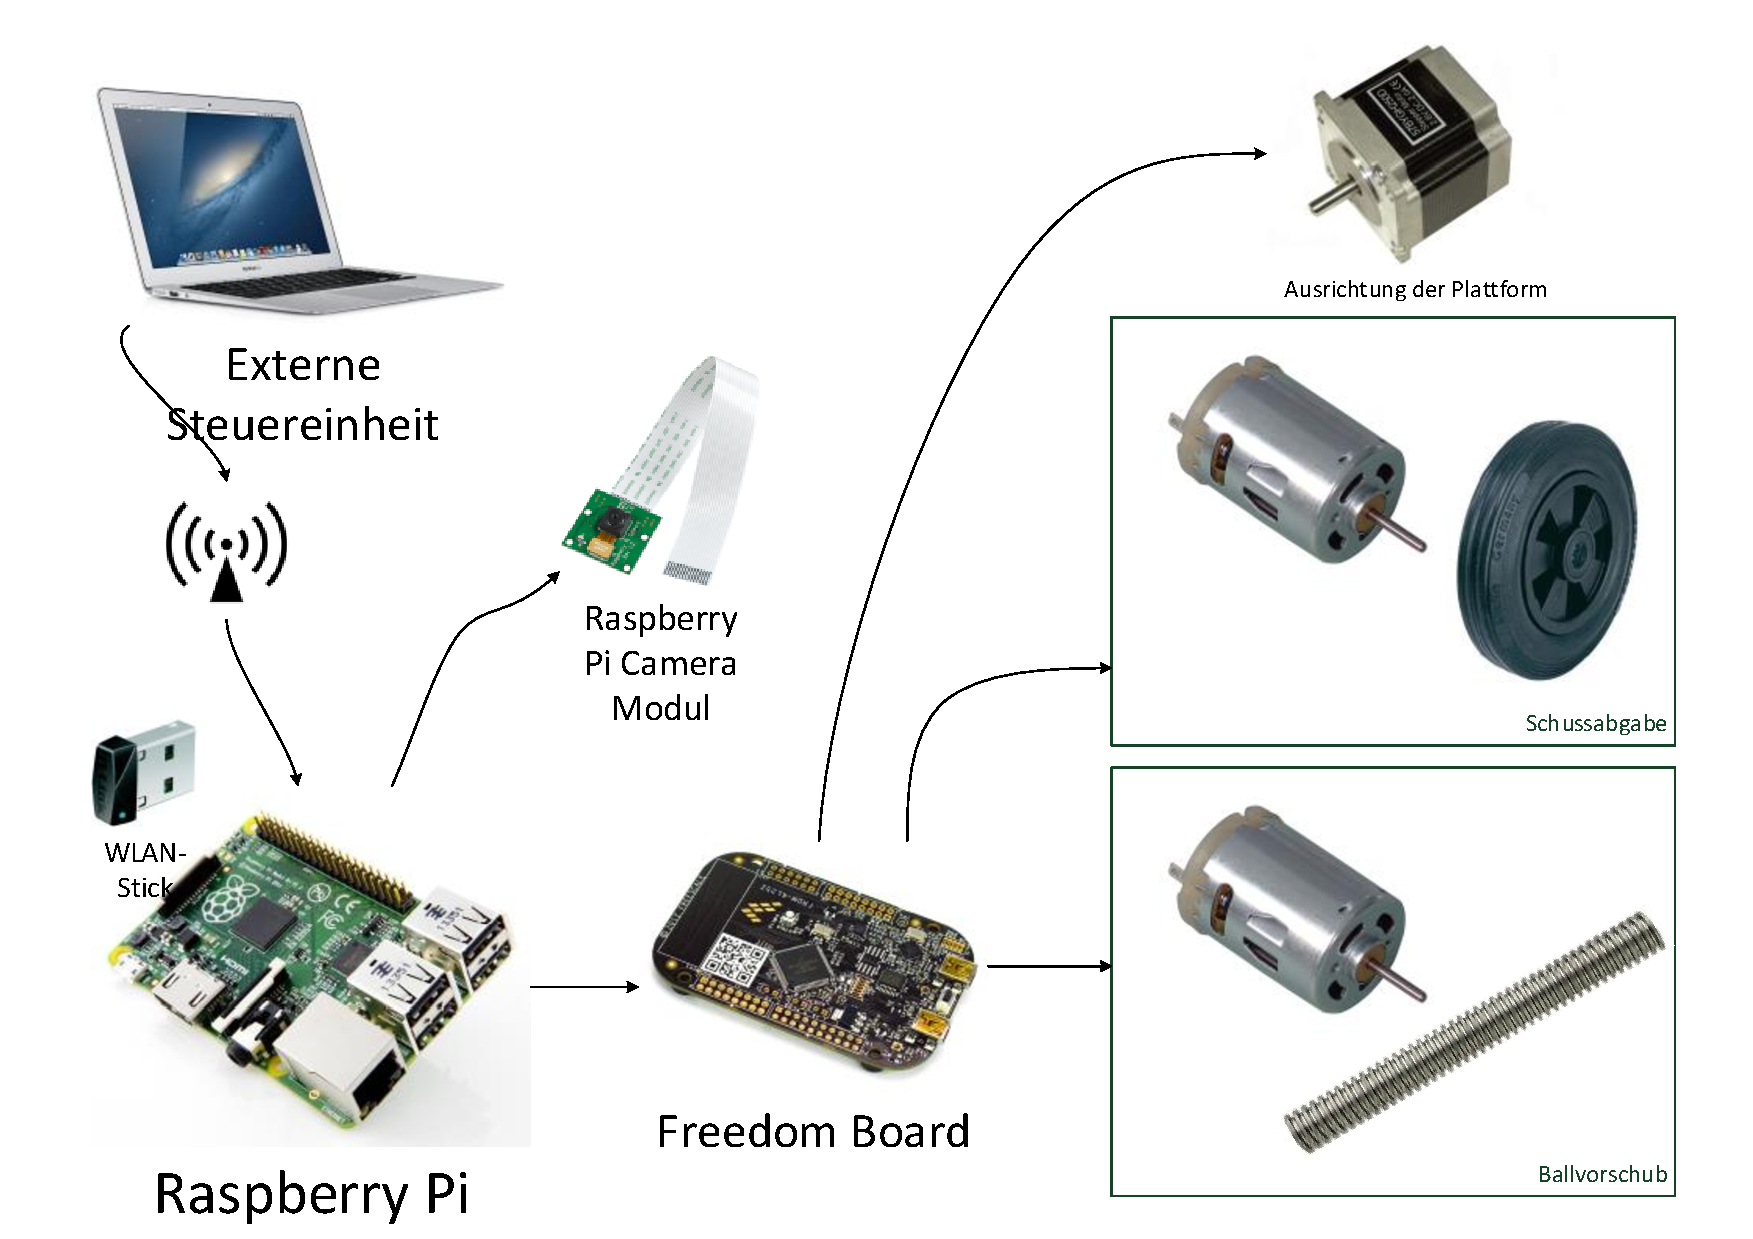
\includegraphics[width=0.9\textwidth]{../../fig/blockdiagramm-fuer-presi.pdf}
	\end{figure}
	
\end{frame}

\begin{frame}
	\frametitle{Übersicht\hfill{}\footnotesize \group}
	\framesubtitle{Aufgaben \& Komponenten}
	\begin{columns}
		\begin{column}{0.5\textwidth}
			\begin{block}{Aufgaben}
				\begin{itemize}
					\item Energieversorgung
					\item Kommunikation
					\item Peripherieansteuerung
					\item Funktionsrealisierung
				\end{itemize}
			\end{block}
			\begin{exampleblock}{Funktionen}
				\begin{itemize}
					\item Einstellen des Azimuts
					\item Einstellen der Wurfdistanz
					\item Nachführen der Wurfobjekte
				\end{itemize}
			\end{exampleblock}
		\end{column}
		\begin{column}{0.5\textwidth}
		\begin{figure}
			\begin{tikzpicture}[node distance=1.5cm]
				\footnotesize
				\node (pwr) [power] {PWR};
				\node (dc) [driver, below of=pwr] {DC};
				\node (bldc) [driver, below of=dc] {BLDC};
				\node (stp) [driver, below of=bldc] {STP};
				\node (mot1) [power, right of=dc] {MOT};
				\node (mot2) [power, right of=bldc] {MOT};
				\node (mot3) [power, right of=stp] {MOT};
				\node (frdm) [logic, left of=pwr] {FRDM};
				\draw[red,thick] (pwr) -| (mot1);
				\draw[red, thick] (mot1) -- (mot2);
				\draw[red, thick] (mot2) -- (mot3);
				\draw[red, thick] (pwr) -- (dc);
				\draw[red, thick] (dc) -- (bldc);
				\draw[red, thick] (bldc) -- (stp);
				\draw[blue, thick, <->] (frdm) |- (dc);
				\draw[blue, thick, <->] (frdm) |- (bldc);
				\draw[blue, thick, <->] (frdm) |- (stp);
				\draw[green, thick, ->] (dc) -- (mot1);
				\draw[green, thick, ->] (bldc) -- (mot2);
				\draw[green, thick, ->] (stp) -- (mot3);
			\end{tikzpicture}
		\end{figure}
		\end{column}
	\end{columns}
\end{frame}

\subsubsection{Fachgruppe ET}
\begin{frame}
	\frametitle{Fachgruppe Elektrotechnik\hfill{}\footnotesize \group}
	\framesubtitle{Motivation \& Ziele}
	\begin{columns}
		\begin{column}{0.5\textwidth}
				\textit{``Denn es ist eines ausgezeichneten
					Mannes nicht würdig, wertvolle Stunden
					wie ein Sklave im Keller der einfachen
					Berechnungen zu verbringen''}
				~ \\ ~ \\
				\hfill{} -- Gottfried Wilhelm Leibniz \\
		\end{column}
		\pause
		\begin{column}{0.5\textwidth}
			\begin{block}{Ziele}
				\begin{itemize}
					\item Synergien nutzen
					\item Fachlicher Austausch
					\item Eigenentwicklungen
					\item OpenHardware
				\end{itemize}
			\end{block}
		\end{column}
	\end{columns}
\end{frame}

\begin{frame}
	\frametitle{Fachgruppe Elektrotechnik \hfill{} \footnotesize \group}
	\framesubtitle{Organisation \& Projekte}
	\begin{columns}
		\begin{column}{0.5\textwidth}
			\begin{block}{github.com/pren-et}
				\begin{itemize}
					\item 7 Contributors
					\item 6 PREN-Teams
					\item 7 Repositories
					\item 3 HW-Projekte
				\end{itemize}
			\end{block}
			\begin{block}{Projekte}
				\begin{itemize}
					\item Motorentreiber für
						\begin{itemize}
							\item Gleichstrommotor (DC)
							\item Brushlessmotor (BLDC)
							\item Schrittmotor (Stepper)
						\end{itemize}
					\item Dokumentationen
				\end{itemize}
			\end{block}
		\end{column}
		\begin{column}{0.5\textwidth}
			\begin{exampleblock}{Teams}
				\begin{tabular}{l l r}
					DC
						& B. v. Büren 	& 19 \\
						& J. Buchli 	& 19 \\
						& F. Kreiliger	& 33 \\
						& E. Mazlagi\'c	& 39 \\
					& & \\
					BLDC
						& D. Winz	& 27 \\
						& Y. Studer	& 32 \\
					& & \\
					Stepper
						& D. Winz	& 27 \\
						& F. Kreiliger	& 33 \\
						& B. Wyss	& 38 \\
				\end{tabular}
			\end{exampleblock}
		\end{column}
	\end{columns}
\end{frame}

\subsubsection{Motoren}
\begin{frame}
	\frametitle{Motoren\hfill{}\footnotesize \group}
	\framesubtitle{Schrittmotor (Stepper) für Turmausrichtung}
	\begin{columns}
		\begin{column}{0.5\textwidth}
			\begin{figure}
				\begin{tikzpicture}[node distance=1.5cm]
					\footnotesize
					\node (frdm) [logic] {FRDM};
					\node (l6480) [driver, below of=frdm] {L6480};
					\node (stp) [power, below of=l6480] {STP};
					\draw[blue, thick, <->] (frdm) -- node[anchor=east] {UART} ($ (frdm) + (0,1) $);
					\draw[blue, thick, <->] (frdm) -- node[anchor=east] {SPI} (l6480);
					\draw[green, thick, ->] (l6480) -- (stp);
				\end{tikzpicture}
			\end{figure}
		\end{column}
		\begin{column}{0.5\textwidth}
			\begin{block}{Eckdaten und Funktion}
				\begin{itemize}
					\item Einstellen des Azimut
					\item Pre-Driver Chip L6480
						\begin{itemize}
							\item Geschwindigkeitsprofil
							\item Microstepping
							\item Schrittüberwachung
							\item Strombegrenzung
							\item Temperaturbegrenzung
						\end{itemize}
				\end{itemize}
			\end{block}
		\end{column}
	\end{columns}
\end{frame}

\begin{frame}
	\frametitle{Motoren \hfill{} \footnotesize \group}
	\framesubtitle{Schrittmotor (Stepper) für Turmausrichtung}
	\begin{columns}
		\begin{column}{0.5\textwidth}
			\begin{figure}
				\centering
				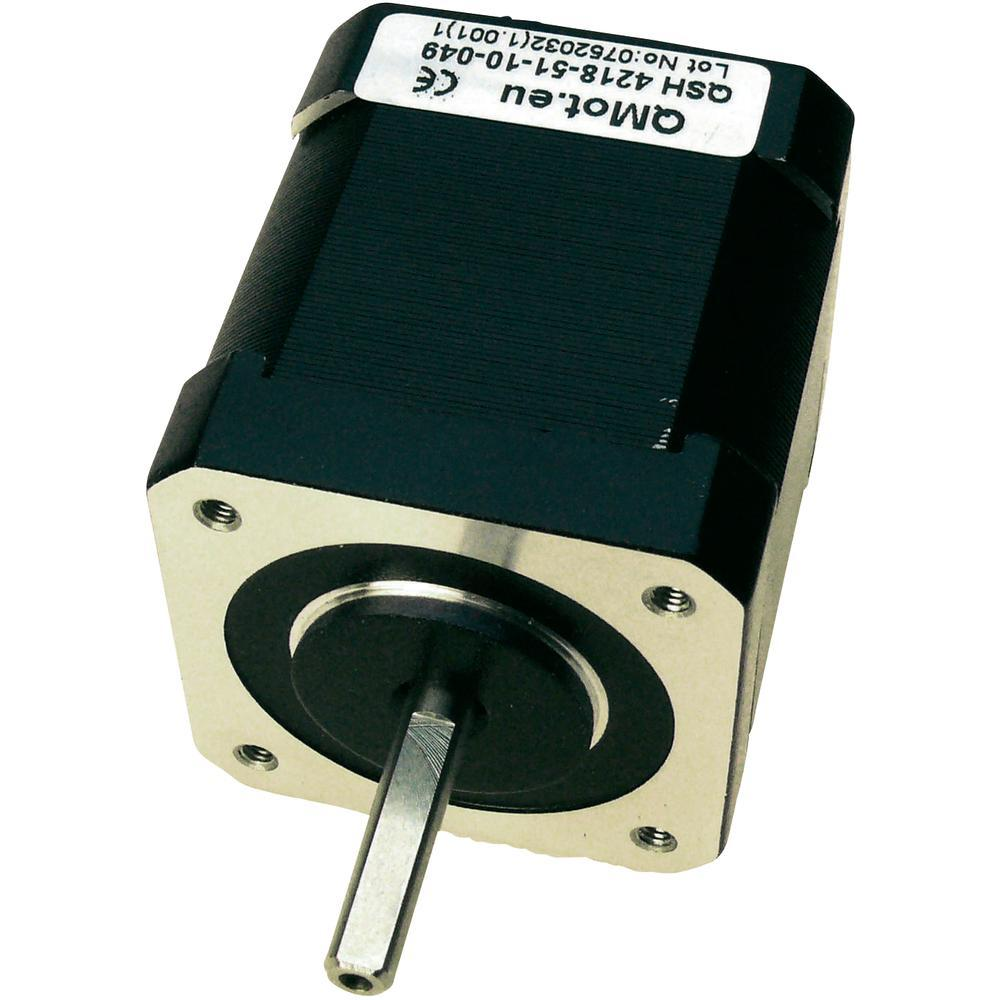
\includegraphics[width=0.9\textwidth]{../../fig/motor/stepper_01.jpg}
				\caption{Schrittmotor QHS4218-51-10-049}
			\end{figure}
		\end{column}
		\begin{column}{0.5\textwidth}
			\begin{block}{Evaluationsergebnisse}
				\begin{itemize}
					\item Modelle fixiert
					\item Energieversorgung unkritisch
					\item Leistungsklasse anpassbar
					\item an der HSLU verfügbar
				\end{itemize}
			\end{block}
			\begin{exampleblock}{Treiberstufe}
				\begin{itemize}
					\item wird mit pren-et entwickelt
					\item Fallback steht bereit
				\end{itemize}
			\end{exampleblock}
		\end{column}
	\end{columns}
\end{frame}

\begin{frame}
	\frametitle{Motoren\hfill{}\footnotesize \group}
	\framesubtitle{Synchronmotor (BLDC) für Ballwurf}
	\begin{columns}
		\begin{column}{0.5\textwidth}
			\begin{figure}
				\begin{tikzpicture}[node distance=1.5cm]
					\footnotesize
					\node (frdm) [logic] {FRDM};
					\node (drv) [driver, below of=frdm] {DRV};
					\node (bldc) [power, below of=drv] {BLDC};
					\draw[blue, thick, <->] (frdm) -- node[anchor=east] {UART} ($ (frdm) + (0,1) $);
					\draw[blue, thick, <->] (frdm) -- node[anchor=east] {SPI} (l6480);
					\draw[green, thick, ->] (drv) -- (bldc);
				\end{tikzpicture}
			\end{figure}
		\end{column}
		\begin{column}{0.5\textwidth}
			\begin{block}{Eckdaten und Funktion}
				\begin{itemize}
					\item Einstellen der Wurfdistanz
					\begin{itemize}
						\item Drehzahl
						\item Leistung
						\item Trägheit
						\item Drehmoment
					\end{itemize}
				\end{itemize}
			\end{block}
		\end{column}
	\end{columns}
\end{frame}

\begin{frame}
	\frametitle{Motoren \hfill{} \footnotesize \group}
	\framesubtitle{Synchronmotor (BLDC) für Ballwurf}
	\begin{columns}
		\begin{column}{0.5\textwidth}
			\begin{figure}
				\centering
				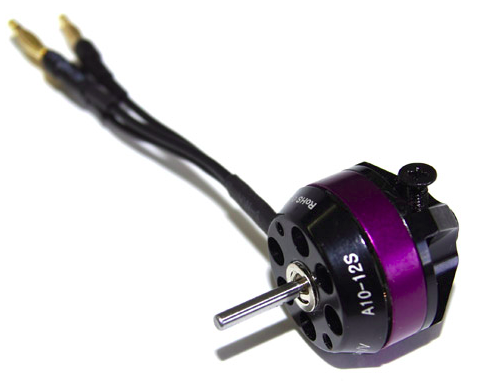
\includegraphics[width=1\textwidth]{../../fig/motor/bldc_02.png}
				\caption{BLDC-Motor A10-12S von Hacker}
			\end{figure}
		\end{column}
		\begin{column}{0.5\textwidth}
			\begin{block}{Evaluationsergebnisse}
				\begin{itemize}
					\item Modelle nicht fixiert
					\item Referenzmodell vorhanden
					\item Energieversorgung kritisch
					\item Leistungsklasse fixiert
					\item an der HSLU nicht verfügbar
				\end{itemize}
			\end{block}
			\begin{exampleblock}{Treiberstufe}
				\begin{itemize}
					\item wird mit pren-et entwickelt
					\item Fallback definiert
				\end{itemize}
			\end{exampleblock}
		\end{column}
	\end{columns}
\end{frame}


\begin{frame}
	\frametitle{Motoren\hfill{}\footnotesize \group}
	\framesubtitle{Gleichstrommotor (DC) für Ballnachführung}
	\begin{columns}
		\begin{column}{0.5\textwidth}
			\begin{figure}
				\begin{tikzpicture}[node distance=1.5cm]
					\footnotesize
					\node (frdm) [logic] {FRDM};
					\node (a3941) [driver, below of=frdm] {A3941};
					\node (dc) [power, below of=a3941] {DC};
					\draw[blue, thick, <->] (frdm) -- node[anchor=east] {UART} ($ (frdm) + (0,1) $);
					\draw[blue, thick, <->] (frdm) -- node[anchor=east] {PWM} (a3941);
					\draw[green, thick, ->] (a3941) -- (dc);
				\end{tikzpicture}
			\end{figure}
		\end{column}
		\begin{column}{0.5\textwidth}
			\begin{block}{Eckdaten und Funktion}
				\begin{itemize}
					\item Nachführung der Bälle
					\item Pre-Driver Chip A3941
						\begin{itemize}
							\item N-Channel H-Brigde
							\item 100\% duty-cycle
							\item fast \& slow decay
							\item anti-shoot-though
							\item einstellbare Totzeit
							\item Diagnose-Pins
						\end{itemize}
				\end{itemize}
			\end{block}
		\end{column}
	\end{columns}
\end{frame}

\begin{frame}
	\frametitle{Motoren \hfill{} \footnotesize \group}
	\framesubtitle{Gleichstrommotor (DC) für Ballnachführung}
	\begin{columns}
		\begin{column}{0.5\textwidth}
			\begin{figure}
				\centering
				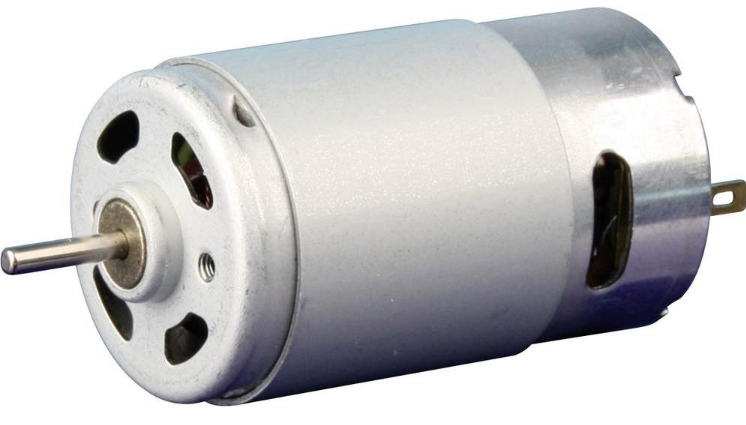
\includegraphics[width=1\textwidth]{../../fig/motor/dc_01.png}
				\caption{Gleichstrommotor X-Drive 555-1 von Motraxx}
			\end{figure}
		\end{column}
		\begin{column}{0.5\textwidth}
			\begin{block}{Evaluationsergebnisse}
				\begin{itemize}
					\item Modelle nicht fixiert
					\item Referenzmodelle vorhanden
					\item Energieversorgung unkritisch
					\item Leistungsklasse wählbar
					\item ggf. and der HSLU verfügbar
				\end{itemize}
			\end{block}
			\begin{exampleblock}{Treiberstufe}
				\begin{itemize}
					\item wird mit pren-et entwickelt
					\item Fallback definiert
				\end{itemize}
			\end{exampleblock}
		\end{column}
	\end{columns}
\end{frame}


\subsubsection{Mikrocontroller}
\begin{frame}
	\frametitle{Mikrocontroller\hfill{}\footnotesize \group}
	\framesubtitle{Freedomboard FRDM-KL25Z}
	\begin{columns}
		\begin{column}{0.5\textwidth}
			\begin{figure}
				\centering
				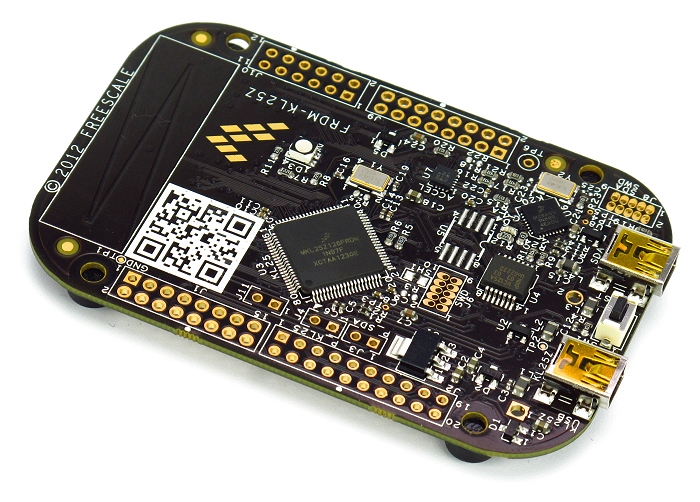
\includegraphics[width=1\textwidth]{../../fig/frdm-kl25z.jpg}
				\caption{FRDM-KL25Z}
			\end{figure}
		\end{column}
		\begin{column}{0.5\textwidth}
			\begin{itemize}
				\item LowLevel-Schnittstelle für
					\begin{itemize}
						\item Motoransteuerung
						\item Sensorik \& Messtechnik
						\item Busse (UART, SPI, I$^2$C)
					\end{itemize}
				\item Programmierung in C
				\item Kommunikation mit UART (USB $\leftrightarrow$ Seriell)
				\item Programmierung mit CW, KDS oder GCC möglich
				\item wird eingesetzt an der HSLU
			\end{itemize}
		\end{column}
	\end{columns}
\end{frame}

\begin{frame}
	\frametitle{Mikrocontroller\hfill{}\footnotesize \group}
	\framesubtitle{Freedomboard FRDM-KL25Z}
	\begin{columns}
		\begin{column}{0.5\textwidth}
			\begin{figure}
				\begin{tikzpicture}[node distance=1.5cm]
					\footnotesize
					\node (linux) [logic] {Linux};
					\node (windows) [logic, right of=linux] {Windows};
					\node (mac) [logic, right of=windows] {MAC};
					\node (usb) [logic, below of=windows] {USB};
					\node (frdm) [logic, below of=usb] {FRDM};
					\node (y) [driver, below of=frdm] {Y};
					\node (x) [driver, left of=y] {X};
					\node (z) [driver, right of=y] {Z};
					\draw[blue, thick, <->] (linux) |- node[anchor=east, very near start] {tty*} (usb);
					\draw[blue, thick, <->] (windows) -- node[anchor=east] {COM} (usb);
					\draw[blue, thick, <->] (mac) |- node[anchor=east, very near start] {cu.*} (usb);
					\draw[blue, thick, <->] (usb) -- node[anchor=west] {USB $\leftrightarrow$ Serial} (frdm);
					\draw[blue, thick, <->] (frdm) -| node[anchor=east, very near end] {SPI} (x);
					\draw[blue, thick, <->] (frdm) -- node[anchor=east] {I$^2$C} (y);
					\draw[blue, thick, <->] (frdm) -| node[anchor=east, very near end] {UART} (z);
				\end{tikzpicture}
			\end{figure}
		\end{column}
		\begin{column}{0.5\textwidth}
			\begin{block}{Wieso Raspberry Pi \& FRDM?}
				\begin{itemize}
					\item Plattformunabhängigkeit
					\item unabhängige, parallele Entwicklung
						\begin{itemize}
							\item INF $\leftrightarrow$ Raspberry Pi
							\item ET $\leftrightarrow$ FRDM
						\end{itemize}
					\item Abstraktion
					\item Modularität
					\item reduzierte Komplexität
					\item Codebasis pren-et
				\end{itemize}
			\end{block}
		\end{column}
	\end{columns}
\end{frame}
